\section{Verification through Sensor Data}
% Verification is a broad topic in buildings that refers to verifying several things about building sensor metadata or through
% the sensor data.  Both cases are related to physical states are relationships that are assumed by the user and are either
% true and empirically observable or not.  If not, the end user or process should be informed and that inconsistencies should
% be immediately addressed.  This is even more of an issues as building begin to reply more and more on software.

% In this section we introduce some of the tools that we use for verification as discuss the 4 types of verification
% that exists in buildings.  We also present an overview approach for 3 of them.

Every system that manages data in the building specifies the building model manually at some point in the life cycle of
the metadata.  Moreover, as the building changes and physical configuration of the building and deployment change,
all changes in the virtual representation of the building are updated manually.  As we move more and more towards
software controlled spaces and system that rely on accurate state capture of the physical environment, it becomes 
of highest important to automate the process that verifies correct configuration specification.

In the architecture we propose we see it as a concurrent process that will be in parallel with all active deployments.
The hierarchical naming scheme explicitly informs the verification process of ``group-by'' relationships between sensors.
Such ``group-by'' relationships typically specify physical relationships, such as grouping sensors that are in the same 
room in the same group, or the same floor in the same group.  Ideally, a verification process could perform several clustering
algorithms, using the empirical data collected from the sensors, to infer such physical relationships.  Most importantly,
it can alert the user when previously statistically clustered sensors no longer show the same \emph{inter-relationship}.

In this chapter, we discuss the analytical underpinning for a verification mechanism that could eventually become a 
component in the StreamFS -- or any other -- building software system.  We introduce the various kinds of verification in depth,
discuss the mathematical tools that help us both formulate and solve related verification problems, and present
results for the empirical verification of various physical relationships between sensors.  In the next section we discuss the various
types of verification, then we describe the tools, methodologies, and results for solving each.

\section{Types of Verification}
There are 3 kinds of verification that we discuss in this section.

\begin{enumerate}
\item \emph{Functional}: verifying whether the behavior of the components in changing.
\item \emph{Spatial}: 	verifying the spatial relationship between components.
\item \emph{Categorical}: verifying the unit of measure and phenomenon being observed.
% \item Value
\end{enumerate}

Before we discuss the details and approach for each, let us first examine the mathematical tools that we
use in our solutions.  Then we discuss each type of verification in more detail.  We give a detailed description 
of the methodology for each and present the results of our analysis.

\subsection{Correlation}
Throughout this work, we make extensive use of the correlation coefficient function defined as: 

\begin{displaymath}
r(X,Y) = r_{X, Y} = \frac{\sum_{i=1}^{n} (X_{i} - \overline{X})(Y_{i} - \overline{Y})}
{\sqrt{\sum_{i=1}^{n} (X_{i} - \overline{X})^2}\sqrt{\sum_{i=1}^{n} (Y_{i} - \overline{Y})^2}}
\end{displaymath}

where $X$, $Y$ are separate sets of values, $n$ is the total number of sample points in 
each set, and $\overline{X}$ is the mean value of $X$ (same for $\overline{Y}$ and Y).  % over the entire sampling period.
For each pair of sensors, we compute the corrcoeff to ascertain the relationship between them.


\subsection{Empirical Mode Decomposition} \label{emd}
Another important tool that we used is empirical mode decomposition.  We use it partition the empirical data is its constituent
sub-signals and examine what those sub-signals tell us about its behavior.  We also use it to examine how signals behave between
one another at certain bands of importance that contain important physical information.

Empirical Mode Decomposition (EMD) \cite{huang:emd1998} is a technique that decomposes a signal and reveals intrinsic patterns, 
trends, and noise.
This technique has been widely applied to a variety of datasets, including climate variables\cite{climate}, medical 
data\cite{blanco:bioMed2008}, speech signals\cite{huang:signalProc2006,hasan:ieeeletter2009}, and image processing~\cite{nunes:vision2005}.
% for example, it helped to uncover the global surface temperature trends\cite{}, solar activity patterns and predicts climate variables .
EMD's effectiveness relies on its empirical, adaptive and intuitive approach.
In fact, this technique is designed to efficiently decompose both non-stationary and non-linear signals without requiring any 
a priori basis functions or tuning.  

EMD decomposes a signal into a set of oscillatory components called intrinsic mode functions (IMFs). 
An IMF satisfies two conditions: (1) it contains the same number of extrema and zero crossings (or differ at most by one); (2) the two 
IMF envelopes defined by its local maxima and local minima are symmetric with respect to zero.  Consequently, 
 IMFs are functions that directly convey the amplitude and frequency modulations.

% EMD is an iterative sifting process that extracts IMFs step by step; each step seeks for the IMF with the highest frequency, then the computed IMF is removed from the data and the residual data are used as input for the next step.
EMD is an iterative algorithm that extracts IMFs step by step by using the so-called sifting 
process \cite{huang:emd1998}; each step seeks for the IMF with the highest frequency by sifting, then 
the computed IMF is removed from the data and the residual data are used as input for the 
next step.
The process stops when the residual data becomes a monotonic function from which no more IMF can be extracted.

We formally describe the EMD algorithm as follows: 
\begin{enumerate}
\item Sifting process: For a current signal $h_0=X$, let $m_0$ be the mean of its upper and lower envelopes as determined from a cubic-spline interpolation of local maxima and minima.
\item The estimated local mean $m_0$ is removed from the signal, giving a first component: $h_1 = h_0-m_0$
\item The sifting process is iterated, $h_1$ taking the place of $h_0$. Using its upper and lower envelopes, a new local mean $m_1$ is computed and $h_2 = h_1-m_1$.
\item The procedure is repeated $k$ times until $h_k=h_{k-1}-m_{k-1}$ is an IMF according to the two conditions above.
\item This first IMF is designated as $c_1 = h_k$, and contains the component with shortest periods. We extract it from the signal to produce a residual: $r_1 = X - c_1$.  Steps 1 to 4 are repeated on the residual signal $r_1$, providing IMFs $c_j$ and residuals $r_j  = r_{j-1}-c_j$, for $j$ from $1$ to $n$.
\item The process stops when residual $r_n$ contains no more than 3 extrema.
\end{enumerate}

The result of EMD is a set of IMFs $c_i$ and the final residue $r_n$, such as: \[X=\sum^{n}_{i=1}c_i+r_n\]
where the size of the resulting set of IMFs ($n$) depends on the original signal $X$ and $r_n$ represents the trend of 
the data (see \emph{IMFs} in Figure~\ref{fig:diagram1}).

For this work we implemented a variant of EMD called Complete Ensemble EMD~\cite{torres:icassp2012}.
This algorithm computes EMD several times with additional noise, it allows us to efficiently analyze signals that have 
flat sections (i.e. consuming no electricity in our case). % and permits us to solve the \emph{EMD mode mixing problem}.

\subsection{Reaggregation of Intrinsic Mode Functions} \label{methodo:corr}
By applying EMD to energy consumption signals we obtain a set of IMFs that precisely describe the devices consumption 
patterns at different frequency bands.  Therefore, we can focus our analysis on the smaller time scales, ignoring the dominant 
patterns that prevent us from effectively analyzing raw signals.

However, comparing the IMFs obtained from different signals is also not trivial,
 because EMD is empirically uncovering IMFs from the data there is no guarantee that the two IMFs $c_i^1$ and $c_i^2$ obtained from two distinct signals $S^1$ and $S^2$ represent data at the same frequency domain.
Directly comparing $c_i^1$ and $c_i^2$ is meaningless unless we confirm that they belong to the same frequency domain.

There are numerous techniques to retrieve IMF frequencies~\cite{IF}.  
In this work we take advantage of the Generalized Zero Crossing (GZC)~\cite{GZC} because it is a simple and robust 
estimator of the instantaneous IMF 
frequency\cite{IF}.
GZC is a direct estimation of IMF instantaneous frequency using critical points defined as the zero crossings and local extrema 
(round dots in Figure~\ref{fig:gzc}).
Formally, given a data point $p$, GZC measures the quarter ($T_4$), the two halves ($T_2^x$), and the four full periods ($T_1^y$), $p$   
belong to (see Figure~\ref{fig:gzc}) and the instantaneous period is computed as:
\[T=\frac{1}{7}\{4T_4+(2T_2^1+2T_2^2)+(T_1^1+T_1^2+T_1^3+T_1^4)\}\]

\begin{figure}
\begin{center}
 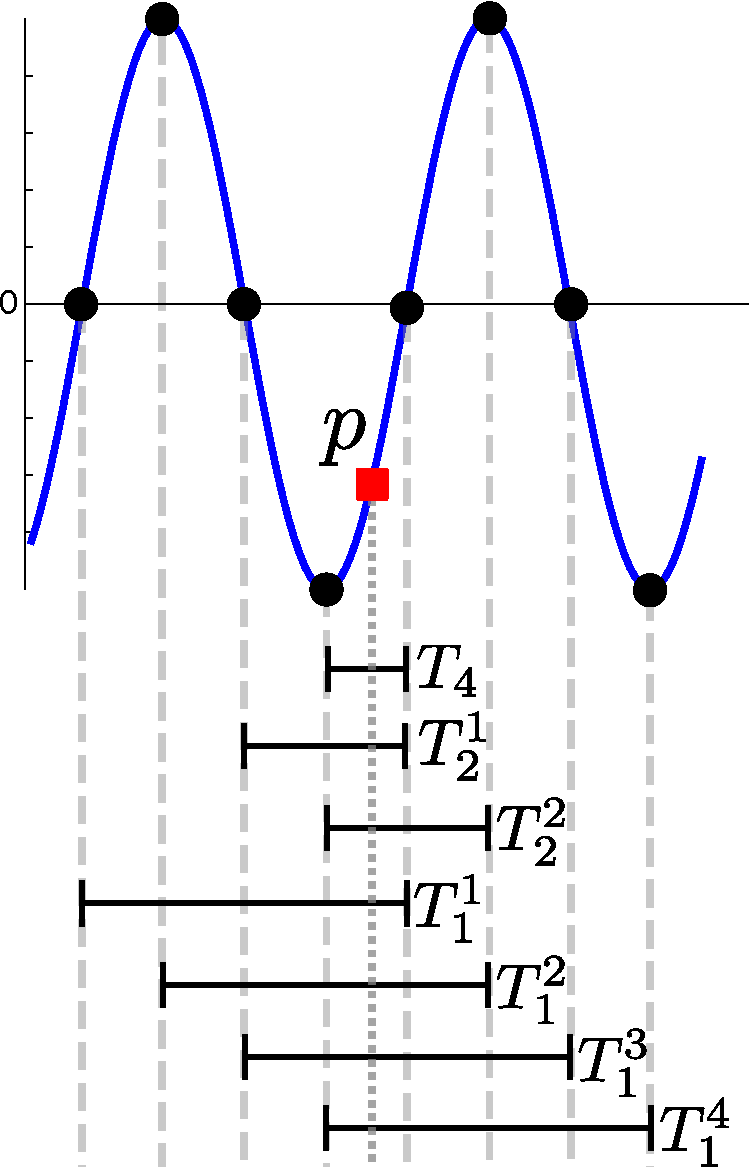
\includegraphics[width=.25\textwidth]{figs/gzc.pdf}
 \end{center}
 \caption{Generalized Zero Crossing: the local mean period at the point $p$ is computed from one quarter period $T_4$, two half periods $T_2^x$ and four full periods $T_1^y$ (where $x=1, 2$, and, $y=1,2,3,4$).}
 \label{fig:gzc}
\end{figure}

Since all points $p$ between two critical points have the same instantaneous period GZC is local down to a quarter period.
Hereafter, we refer to the time scale of an IMF as the average of the instantaneous periods along the whole IMF.
Because the time scale of each IMF depends on the original signal, we propose the following to efficiently compare IMFs from different signals.
We cluster IMFs with respect to their time scales and partially reconstruct each signal by aggregating its IMFs from the 
same cluster.  Then, we directly compare the partial signals of different devices.

EMD yields distinct components in different time scales and we compute the instantaneous frequencies \cite{IF} of IMFs using Generalized Zero-Crossing \cite{GZC}.  We break the time scales into four frequency bands:
\begin{itemize}
\item High Frequency: a time scale smaller than 30 minutes, mainly reflecting the operation characteristics of devices and noise in system. 
\item Medium Frequency: a time scale between 30 minutes and 6 hours, which is within the time span of daily activities inside a building.
\item Low Frequency: a time scale between 6 hours and 7 days. %This category usually captures patterns repeated in a longer cycle, say, days. 
\item Residue: everything has a time scale longer than 7 days and shows long-term patterns, such as seasonal changes.
\end{itemize}

Later in this thesis we will explain how we use the medium-frequency band for both spatial verification and functional verification.  We discuss
the 4 types of verification in the next section.







\subsection{Functional Verification}% With Strip, Bind, and Search}
% A typical large building contains thousands of sensors, monitoring the HVAC system, lighting, and other operational sub-systems.
With an increased push for operational efficiency, operators are relying more on historical data processing to uncover opportunities for energy-savings.
However, they are overwhelmed with the deluge of data and seek more efficient ways to identify potential problems.
In this thesis, we present an approach called the Strip, Bind and Search (SBS); a method for uncovering abnormal 
equipment behavior and in-concert usage patterns.
SBS uncovers relationships between devices and constructs a model for their usage pattern relative to other devices.
It then flags deviations from the model. 
% Unlike other approaches, SBS requires no a priori knowledge about the building.


The intuition behind the proposed approach is that each service provided by the building requires a minimum subset of devices.
The devices within a subset are used at the same time when the corresponding service is needed and a savings opportunity is characterized by the partial activation of the devices.
For example, office comfort is attained through sufficient lighting, ventilation, and air conditioning.
These are controlled by the lighting and HVAC (Heating, Ventilation, and Air Conditioning) system.
%controlled by the lighting system and air conditioner.% the light and air conditioning.
Thus, when the room is occupied both the air conditioner (heater on a cold day) and lights are used together and should be turned off 
when the room is empty.
In principle, if a person leaves the room and turns off \emph{only} the lights then the air conditioner (or heater) is a source of electricity waste.

Following this basic idea we propose \emph{Strip, Bind and Search} (SBS), an unsupervised methodology that systematically detects electricity waste.
Our proposal consists of two key components:
% \begin{enumerate}
%  \item The strip and bind method (SBM) mines raw sensor data, identifying devices that are used in concert.
%  It uncovers the devices relationships by looking at the correlation of their activities. 
%  Therefore it allows us to differentiate the devices that are used all together (high correlation), devices used independently (no correlation) and the mutually exclusive usages of devices (negative correlation).
%  \item The anomaly detector monitors devices relationships over time and reports misbehaving devices.
%  It learns the devices normal usages using a robust and longitudinal analysis of the building data and detect anomalous usages that stand for electricity wastes.
% \end{enumerate}

\begin{description}
 \item[Strip and Bind] The first part of the proposed method mines the raw sensor data, identifying inter-device usage patterns. % that are typically used in concert to provide a service.
We first \emph{strip} the underlying traces of occupancy-induced trends.  Then we \emph{bind} devices  whose underlying behavior is highly correlated. %, by placing them into a correlated device set.
 %  Then
 % It uncovers the devices relationships by looking at the correlation of their activities. 
 This allows us to differentiate between devices that are used together (high correlation), used independently (no correlation), and used mutually exclusively (negative correlation).
 \item[Search] The second part of the method monitors devices relationships over time and reports deviations from the norm.  % misbehaving devices.
 It learns the normal inter-device usage using a robust, longitudinal analysis of the building data and detect anomalous usages.  Such abnormalities usually present an opportunity to reduce electricity waste or events that deserve careful attention (e.g. faulty device).
 % that may represent that stand for electricity wastes.
\end{description}

SBS overcomes several challenges.  First, 
%The main challenge we overcame with our approach is uncovering the device relationships from numerous, 
noisy sensor traces that all share a similar trend, making direct correlation analysis non-trivial.
%The main difficulty in this approach is to uncover the devices relationship from the numerous and noisy sensor traces. 
Device energy consumption is mainly driven by occupancy and weather, all the devices display a similar daily pattern, in 
roughly overlapping time intervals and phases.
%and seem to be used all at once.
Therefore, one of the main contributions of this work is uncovering the intrinsic device relationships by filtering out the 
dominant trend.  For this task we use 
%% Romain
%This is achieved using a signal processing technique that exhibit the inherent characteristics of time series data, the 
Empirical Mode Decomposition \cite{huang:emd1998}, a known method for de-trending time-varying signals.
%% Romain

Another key contribution of this work is in using SBS to practically monitor building energy consumption.
Moreover, the proposed method is easy to use and functions in any building, as it does not require prior knowledge of the building nor extra sensors.  
It is also tuned through a single intuitive parameter.  %which parameter?

% In the rest of this paper, we detail the mechanisms of SBS (Section \ref{methodo}) before evaluating it with real data (Section \ref{eval}) then we discuss different outcomes of the proposed methodology (Section \ref{discussion}) and conclude.


\subsection{Spatial Verification}

Typically, placement information is embedded in the name or associated metadata for each sensor in the building.
These are used to group sensors by location.  For example, in our building data, all sensors that contain the string
 `410' in their name are in room 410.  Processes typically group streams in this fashion: using regular-expression matching 
or field-matching queries on the characters in the sensor name or metadata.  If these are not updated to reflect changes
then such group-by query results will not accurately represent true spatial relationships.  
% Fontugne et al.~\cite{IOT}
We observe that spatial associations can be derived empirically.  We start with this approach in our 
work and explore, more deeply, the extent to which it can be used 
as a verification tool for corroborating the groups constructed from character-matching queries.  We refer
to this process as \emph{spatial verification}.


\begin{figure*}[ht!]
\centering
    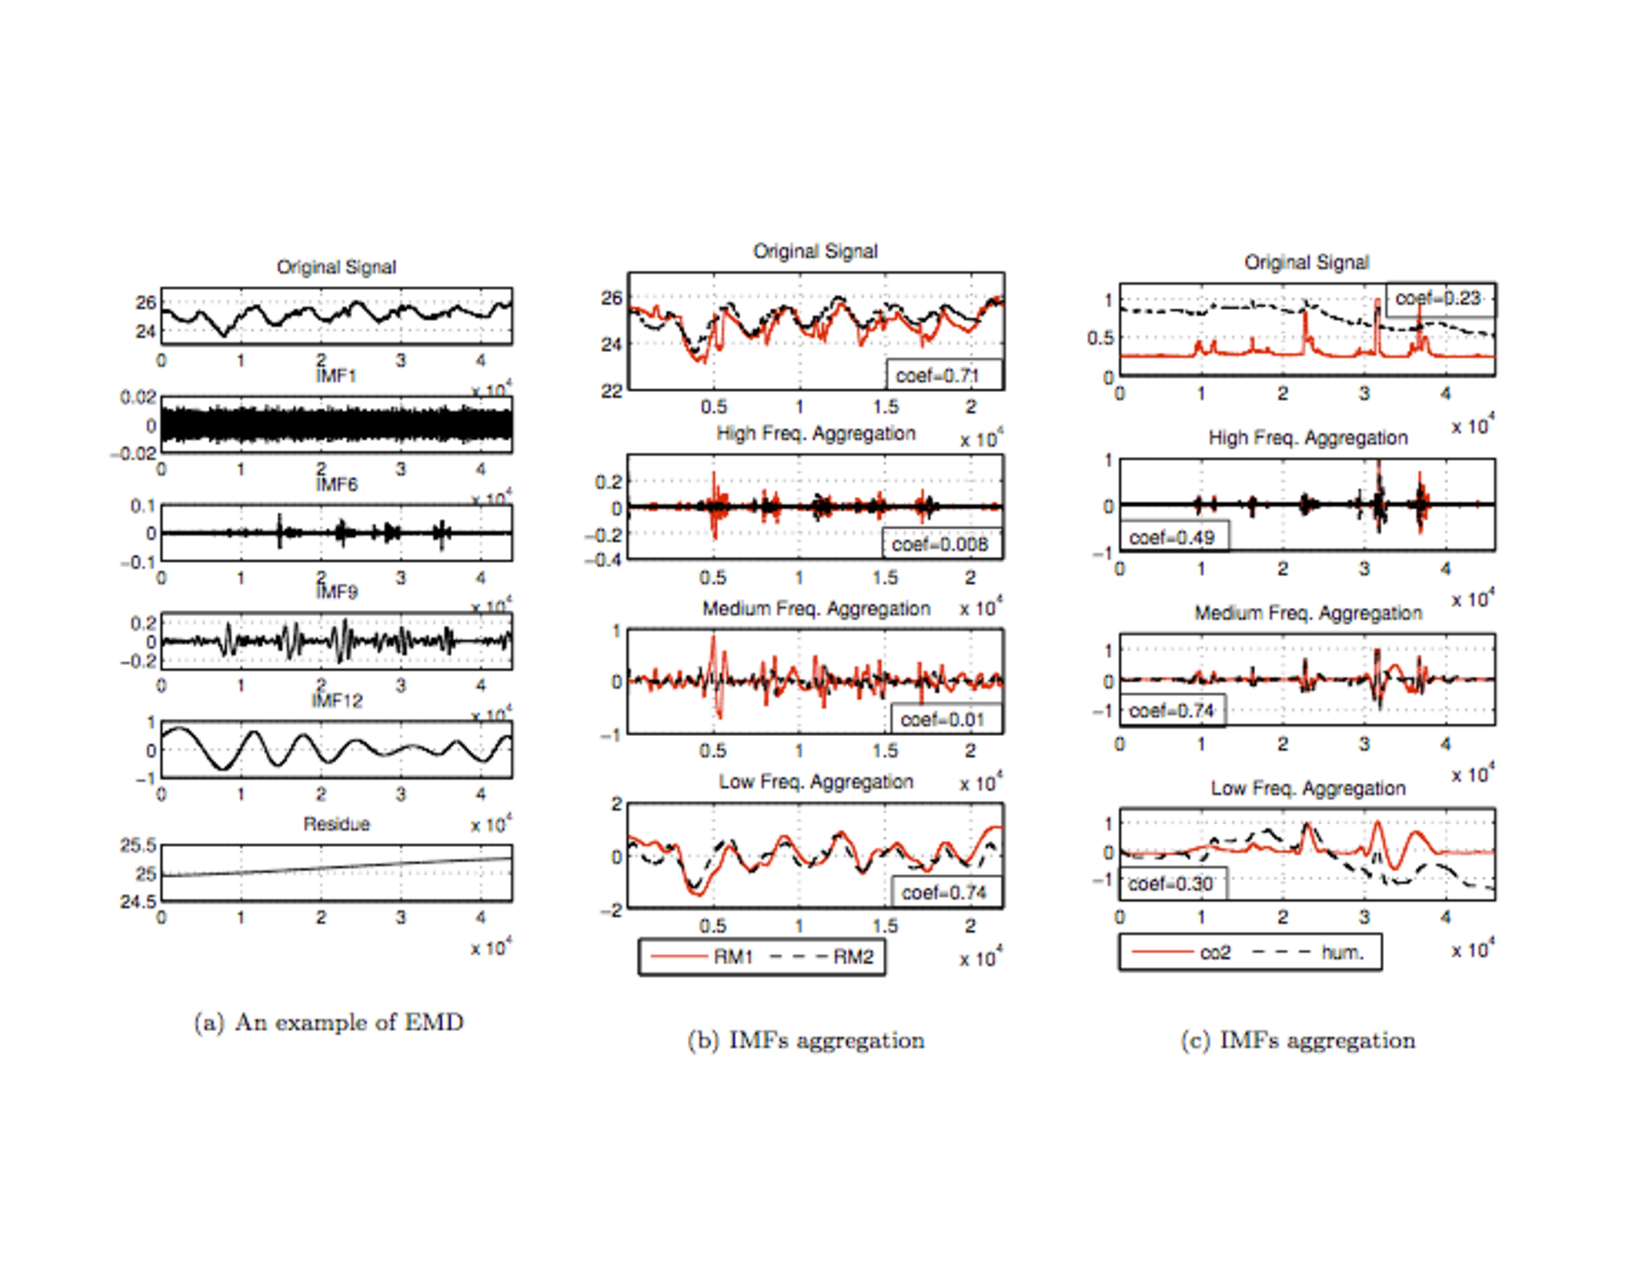
\includegraphics[width=0.95\textwidth]{figs/IMFReAggExample}
\caption{(a) EMD decomposes a signal and exposes intrinsic oscillatory components; (b) Aggregation of IMFs within a pre-defined frequency range makes seemingly similar signals from different locations more distinguishable; (c) IMF aggregation makes seemingly distinct signals of different sensors in the same room show high correlation.}
\end{figure*}

% We investigate the utility of empirical mode decomposition (EMD) to identify intrinsically
% correlated usage patterns among sensors in a large deployment.  We use data collected from almost $700$
% sensors in a 12-story building measuring power, pressure, temperature, and other physical
% phenomena.  We discover that doing a correlation analysis on the raw traces does not discriminate well enough
% to identify meaningful relationships between sensors.  We correlate the trace from a pump with the rest of
% the sensor traces and find that simple correlation filters only $50\%$ of the sensors as being correlated
% with the behavior of the pump. 
% In contrast, by running the correlation analysis on the constituent frequencies extracted by
% the EMD process, we filter out over $99\%$ of the sensors as being correlated -- with the highest correlation coming 
% from sensors that serve the same room as the pump.  We believe our approach can be used to 
% construct inter-device correlation models that can help understand and identify misbehaving or inefficient
% usage patterns.

% We present results for correlating usage patterns across a large number of sensors
% in a single deployment.  We analyze data from a 12-story office building at the University of Tokyo.  
% The deployment consists of almost 700 sensors monitoring a broad range of devices inside and outside 
% the building.  Our initial observations and results include the following:

% \begin{enumerate}
% \item Raw-trace correlation analysis is too strongly influenced by the common low-frequency trends in the data
% 	to identify meaningful relationships.
% \item Using a technique called empirical model decomposition (EMD)~\cite{huang:emd1998} removes this 
% 		 trend and helps identify truly correlated sensor traces.
% \item We can construct clusters of correlated sensors that are spatio-temporally correlated, \emph{without
% 		a priori knowledge of their placement}.
% \end{enumerate}



% Prior work~\cite{IOT} makes use of a technique called Empirical Mode Decomposition (EMD)~\cite{EMD} to statistically cluster correlated
% usage patterns.  Sensors close to each other show strong statistical correlations while sensors further apart show weaker correlations.  
% The main parameter in their approach, the correlation threshold, is explored to demonstrate how it relates to characteristic spatial patterns
%  in the sensor feeds.  However, they do not characterize the threshold as it relates to physical configuration.
% Fontugne et al.~\cite{SBS} expand the work by applying EMD to uncover functional device patterns.  They develop
% an unsupervised learning method to model normal usage patterns and apply an anomaly detection algorithm to alert when patterns
% have deviated from the norm.  The methodology used in their work divides raw signals into four separate frequency bands
% and shows the medium band to carry the most spatial information.

% In this section, we explore the threshold parameter in~\cite{IOT} more deeply, in order to move towards automatic spatial clustering, 
% to be used as a form of verification. We use EMD and the intrinsic mode function (IMF) re-aggregation methodology described in~\cite{SBS}, with some modifications, to statistically analyze the threshold parameter
% and its relationship to spatial separation in a building.  We explore the hypothesis that \emph{a statistical boundary, analogous to a physical one,
% exists and is empirically discoverable}.
% We conduct an empirical analysis on the data collected from 15 sensors in 5 rooms over a one-month period.  Our study makes the following contributions:

% \begin{itemize}
% \item We corroborate the results in~\cite{IOT}, verifying the spatial correlation pattern in a very different building.
% \item We characterize the correlation coefficient (corrcoeff) distribution of sensors in the same room and different rooms and validate our existence hypothesis for this preliminary sample.
% \item We demonstrate that the statistical boundary between sensors in various rooms converges to a similar value and this value generalizes across rooms in this study.
% \item We show the tradeoff between the true and false positive rate inherent to threshold selection. We also show that our method improves the classification accuracy from 80\% to 93.3\%.
% \end{itemize}

% Our results are promising yet preliminary.  We are able to find a statistical separation across a small number of rooms, quite well.
% Our study, however, does not explore the extent to which the physical separation affects the results.  Certainly for rooms that
% are far apart we observe a statistical distinction using our methodology.  However, we also find that in some cases, our approach
% does not work as well.  We discuss the approach and results in the rest of the paper, followed by a short discussion and future work.


We start our analysis by extending the methodology used for functional verification, based on empirical mode decomposition (EMD).  
In our analysis, we collect traces from several sensors and run EMD on them.  This produces a set of 
``intrinsic mode functions'' (IMF), which we separate by frequency range and re-aggregate them into distinct bands.
Then, we inspect the relationship between the sensors by computing the corrcoeff within a particular band, which 
gives us the spatial information we are interested in. 
Finally, we separate the result set into sub-sets, and closely examine their statistical characteristics. 
% Before describing our methodology in detail, we introduce some definitions and notation.



\subsection{Categorical Verification}
Categorical verification is the ability to cluster sensor traces by the type of sensor that it (i.e. its unit of measure) and the thing it is measuring.
Ideally we should be able to separate feeds that are measuring different physical attributes and/or are placed in different parts of the building.
For example, if there are sensors measuring temperature in a pipe and temperature in a room we should be able to separate them from one another as well
as separate them from sensor pressuring pressure in a valve.  We will show that this can be by examining their distribution and for 
small data sets with different sensor our approach works quite well, however we present some challenges in a large, more realistic deployment
data set and we discuss why it is so challenging to deal with.


% \subsection{Value Verification}
% Value verification used a physical model to verify that the value observed in the given context is producing values that agree with the model
% that is based on first-principles.  We do not explore this problem in this thesis and leave it for future work.


